%\documentclass[twocolumn,10pt,letterpaper]{extarticle}
\documentclass{sig-alternate-10pt}


\usepackage{amstext}
\usepackage{algorithm}
\usepackage{algorithmic}
\usepackage{textcomp}
\usepackage{cite}
\usepackage[normalem]{ulem}

%%% Set these variables appropriately
%%%
%% Note:  Authors is hardcoded below, this line only used for the PDF info
%\newcommand{\AUTHORS}{Authors}�
%\newcommand{\TITLE}{Coexisting with Wireless Microphones in a TV Channel}
%\newcommand{\KEYWORDS}{}
%\newcommand{\CONFERENCE}{NSDI 2011}
%\newcommand{\PAGENUMBERS}{no}       % "yes" or "no"
%\newcommand{\TOAPPEAR}{no}
%\newcommand{\COLOR}{yes}
%\newcommand{\showComments}{yes}
%\newcommand{\comment}[1]{}
%\newcommand{\onlyAbstract}{no}
%\newcommand{\ignore}[1]{}
%\newcommand{\strober}{MicProtector}

%%%%%%%%%%%%%%%%%%%%%%%%%%%%%%%%%%%%%%%%%%%%%%%%%%%%%%%%%%%%%%%%%%%%%

%%%
%%%  Page Setup
%%%
\special{papersize=8.5in,11in}
\setlength{\pdfpagewidth}{8.5in}
\setlength{\pdfpageheight}{11in}
%
%\usepackage{ifthen}
%\ifthenelse{\equal{\PAGENUMBERS}{yes}}{%�
%            left=1in,right=1in,top=1in,
%            footskip=0.5in,bottom=1in,     % Room for page numbers
%            columnsep=0.25in
%            ]{geometry}
%}{%
%\usepackage[noheadfoot,left=0.75in,right=0.85in,top=0.75in,
%            footskip=0.5in,bottom=1in,
%            columnsep=0.25in
%        ]{geometry}
%}

%%%
%%%  Captions
%%%
%\usepackage[font=bf]{caption}
%\usepackage[font=bf,aboveskip=0pt]{caption} % SPACE

%%%
%%%  Section headings
%%%
%\usepackage{titlesec}

%%%
%%%  Lists
%%%
%\usepackage{enumitem}
%\setlist{itemsep=0pt,parsep=0pt}             % more compact lists

%%%
%%%  Header / Footer
%%%
%\usepackage{fancyhdr}
%\renewcommand{\headrulewidth}{0pt}

%\ifthenelse{\equal{\PAGENUMBERS}{yes}}{%
%  \pagestyle{plain}
%}{%
%  \pagestyle{empty}
%}

%%%
%%%  Bibliography
%%%
%\usepackage[numbers]{natbib}

%%%
%%%  Footnotes / Endnotes
%%%
\interfootnotelinepenalty=10000  % Split footnotes are annoying

%%%
%%%  Tables
%%%
\usepackage{booktabs}
\usepackage{color}
\usepackage{colortbl}

\usepackage[table]{xcolor}
\usepackage{multirow}

%%%
%%%  Fonts
%%%
\usepackage{mathptmx}                        % Times/Times-like math symbols
\usepackage{courier}
%\usepackage[scaled=0.92]{helvet}

%%%
%%%  PDF setup
%%%
%\ifthenelse{\equal{\COLOR}{yes}}{%
%  \usepackage[colorlinks]{hyperref}%         % for online version
%}{%
%  \usepackage[pdfborder={0 0 0}]{hyperref}%  % for paper (B&W) version
%}
\usepackage{url}

%\hypersetup{%
%pdfauthor = {\AUTHORS},
%pdftitle = {\TITLE},
%pdfsubject = {\CONFERENCE},
%pdfkeywords = {\KEYWORDS},
%bookmarksopen = {true}
%}

%%
%% Figure placeholder macros
%%

%\definecolor{placeholderbg}{rgb}{0.85,0.85,0.85}
%\newcommand{\placeholder}[1]{%
%\fcolorbox{black}{placeholderbg}{\parbox[top][1.5in][c]{0.95\columnwidth}{#1}}}


%%%
%%%  Misc
%%%
\usepackage{graphicx}
\usepackage{subfigure}

%%%
%%%  Sample ACM Copyright Block
%%%
%\usepackage{float}
%\newfloat{acmcr}{b}{acmcr}
%\newcommand{\acmcopyright}{%
%\begin{acmcr}
%\parbox[b]{20pc}{%
%\footnotesize
%Permission to make digital or hard copies of all or part of this work
%for personal or classroom use is granted without fee provided that
%copies are not made or distributed for profit or commercial advantage
%and that copies bear this notice and the full citation on the first
%page.  To copy otherwise, to republish, to post on servers or to
%redistribute to lists, requires prior specific permission and/or a fee.
%
%{\em Conference}, Month Date--Date, Year, Location\\
%Copyright 200X ACM X-XXXXX-XX-X/XX/XX ...\$5.00}
%\end{acmcr}}

%%%
%%%  Comments
%%%
\newcommand{\note}[2]{
    \textcolor{#1}{#2}
}

   \newlength{\realbaselineskip}
\setlength{\realbaselineskip}{\baselineskip}
\newcommand{\changespacing}[1]{\setlength{\baselineskip}{#1\realbaselineskip}}

\newcommand{\george}[1]{\note{magenta}{George: #1}}
\newcommand{\chris}[1]{\note{green}{Chris: #1}}
\newcommand{\thomas}[1]{\note{blue}{Thomas: #1}}
\newcommand{\onur}[1]{\note{red}{Onur: #1}}
\newcommand{\srini}[1]{\note{red}{Srini: #1}}

\newcommand{\squishlist}{
   \begin{list}{$\bullet$}
    { \setlength{\itemsep}{0pt}      \setlength{\parsep}{3pt}
      \setlength{\topsep}{3pt}       \setlength{\partopsep}{0pt}
      \setlength{\leftmargin}{1.5em} \setlength{\labelwidth}{1em}
      \setlength{\labelsep}{0.5em} } }

\newcommand{\squishlisttwo}{
   \begin{list}{$\bullet$}
    { \setlength{\itemsep}{0pt}    \setlength{\parsep}{0pt}
      \setlength{\topsep}{0pt}     \setlength{\partopsep}{0pt}
      \setlength{\leftmargin}{2em} \setlength{\labelwidth}{1.5em}
      \setlength{\labelsep}{0.5em} } }

\newcommand{\squishend}{
    \end{list}  }





% This needs to be the last thing before \begin{document}
%\usepackage{microtype}  % SPACE

%%%%%%%%%%%%%%%%%%%%  START DOCUMENT  %%%%%%%%%%%%%%%%%%%%%%%%
\begin{document}

\date{}
\title{\LARGE \textbf{Heterogeneous-Aware Spectrum Assignment and Management}}
\author{{\large Paper \#blah}\\
%{\em Affiliations}
}

\maketitle

% !TEX root = main.tex

\abstract{
Heterogeneity has become an increasing problem in the wireless spectrum, breaking down spectrum sharing, exacerbating interference, and making highly inefficient use of already scarce spectrum.  Coexistence techniques can alleviate such interference, however they are difficult to deploy (requiring changes across many layers), often incurring overhead, and they are typically short-lived due to rapid changes in technologies and standards.  While spectrum management can be a more efficient and long-term solution, current models have remained relatively homogeneous and Wi-Fi centric.

In this paper, we present a novel heterogeneous spectrum assignment model to properly organize current environments and reduce interference within them.  This model incorporates differences in the physical and MAC layers of radios in the environment, as well as their spatial dynamics (i.e., what interferes with what).  We represent these properties using an annotated hypergraph, and introduced a non-linear mixed integer program to find efficient heterogeneous spectrum organizations.  Results from a heterogeneous testbed show the spectrum organizations to be highly efficient, as well as able to account for various PHY and MAC conflicts.

%To represent the environment, we introduce a hypergraph-based model.  Then, leveraging the hypergraph, we 

% To do so, we first introduce a hypergraph-based model to accurately represent a heterogeneous environment and properties of it.  Then, we introduce a metric to estimate the performance of a network

%Our model is generic, yet descriptive.  By maintaining generic

%Proper heterogeneous spectrum management can be a more efficient and long-term solution
%
% techniques can alleviate such interference, however these approaches are difficult to deploy and
%
%In this paper, we present a heterogeneous spectrum assignment model and algorithm towards a long term solution to cross-technology interference.  }

% !TEX root = main.tex

\section{Introduction}

No single radio design or set of wireless protocols can meet the specific needs and constraints of the many applications for wireless technology.  As a result, heterogeneity has become a fundamental property of the wireless spectrum.  Differences in physical layers, MAC layers, transmission powers, and spectral bandwidths are driven by these varying application requirements.  Unfortunately, differences in these properties break down spectrum sharing and can lead to significant interference between heterogeneous technologies~\cite{buzzbuzz,wifinet,airshark,rfsmog}. 

One popular approach to prevent such heterogeneous interference is to develop coexistence techniques between pairs of technologies (e.g., between Wifi and ZigBee~\cite{buzz buzz}, or Cordless Phones and Wifi~\cite{rfsmog}). While coexistence techniques can alleviate interference, this general approach requires $N^2$ solutions between all technology pairs (where $N$ is growing).  Additionally, coexistence techniques are difficult to deploy.  They incur overhead, changes are often needed at lower layers (e.g., PHY \& MAC), and rapid changes to  technologies and standards can make such solutions short-lived.

% require modifications to layers that are implemented in the radio hardware (e.g., PHY \& MAC), they can , they incur overhead and complexity, and they are short lived due to wireless technologies rapidly changing.  
 
To the contrary, \emph{heterogeneous spectrum management can be an efficient and long-term solution}.  Ideally, the approach frequency-isolates incompatible technologies when possible, and otherwise intelligently places them together where they will receive and generate the least interference.  This approach has several key benefits:  1) It does not require changes to the protocols or radios, 2) It is a ``single solution'' (i.e., it does not require a unique solution/technique for each pair of technologies), and 3) It can continue to be applied to future technologies if the model is generic.

% If modeled and applied generically (i.e., without specifics to any single technology), the approach can 
%
%does not incur overhead, require pairwise solutions, and 
%
%While this approach can have greater longevity, it is non-trivial
%
%While we have made strides in gathering the required information about heterogeneous radios and their interference (e.g., through monitors such as Airshark, DOF, RFDump, and WifiNet \cite{airshark,dof,rfdump,wifinet}), \emph{our spectrum assignment models and algorithms are predominantly homogeneous and Wifi-centric}. 
%
%
%At the most basic level, spectrum management has required information about where signals go and what they interfere with.

Recently, monitors such as Airshark, DOF, RFDump, and WifiNet \cite{airshark,dof,rfdump,wifinet} have made strides in gathering the required environmental information about heterogeneous radios and their interference which makes spectrum management possible.  \emph{However, our spectrum assignment models and algorithms are predominantly homogeneous and Wifi-centric, unable to represent and use such information to efficiently (re)assign heterogeneous spectrum.}  



%For example, historical models such as graph coloring~\cite{utilfair,unified} are unable to represent differences in MAC layers and differences in spectrum usage (i.e., bandwidths and channels).  Referring to Figure~\ref{fig:color_example}, we show two possible ways to color a set of Wifi and ZigBee channels.  In \emph{Scenario 1}, all possible sets of channels (independent of technology) are given different colors.  When applying this scenario, traditional coloring algorithms will distribute ZigBee networks within Wifi channels under the assumption that they do not conflict (they have different colors).  This is agnostic to their destructive MAC interaction.  In \emph{Scenario 2}, if one colors all channels in the spectrum block the same (independent of bandwidth), the algorithm cannot properly distribute the sub-channels (e.g., ZigBee's, which have the same color).
%
%\begin{figure}[t]
%\centering
%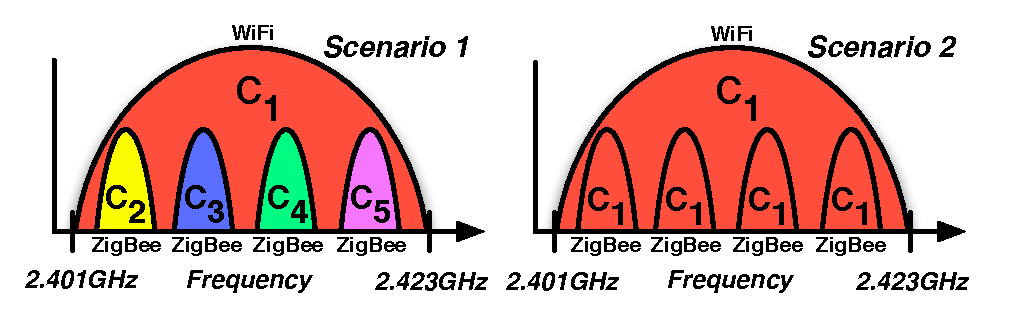
\includegraphics[width=3in]{figures/coloring_single}
%\vspace{-0.2in}
%\caption{\label{fig:color_example} \small Historical spectrum assignment models break-down under heterogeneity, as we illustrate with this graph coloring example.}
%\center
%\vspace{-0.3in}
%\end{figure}


%asymmetric power relationships, or the effects of differences in MAC layers, as commonly found 
%
%For example, historical models such as graph coloring cannot represent 
%
%%For example, graph coloring is unable to model 
%
%%As antidotal evidence, consider spectrum management between 
%
%For example, historical models such as graph coloring 
%
%Historical models such as graph coloring are unable to represent the critical differences in heterogeneous networks.  For example, whether 

%However, spectrum assignment models have remained fairly homogeneous and Wifi-centric.

%This requires knowledge of which heterogeneous devices are within range of each other in the environment, and a spectrum assignment model which, using such information, (re)organizes devices in the spectrum towards better efficiency.

%:  1)  Heterogeneous and spatial information about the environment, i.e., where heterogeneous signals go and what they interfere with, and 2)  A spectrum assignment model that is \emph{accurate} and \emph{general} enough to be applicable to many technologies that consistently evolve.

%An ideal heterogeneous spectrum assignment model should be:  1) \emph{Generic} such that it is not tied heterogeneous spectrum assignment model needs to:  1)  

More recent work, albeit heterogeneous, remains Wifi-centric: non-Wifi transmitters are treated as static interferers, their interference is estimated on the Wifi network, and Wifi channels can be re-assigned (e.g., WifiNet~\cite{wifinet}).  Interference is \emph{not} estimated between all pairs of heterogeneous networks, and management only occurs on the Wifi network.

An ideal model needs to be able to represent differences in properties of heterogeneous networks and devices, it needs to be comprehensive (i.e., not Wifi-centric), and importantly: it should be \emph{generic, yet descriptive}.  In being generic, the model should not include specifics of technologies (e.g., of Wifi or Bluetooth); it should only use primitives e.g., \emph{is device X in range of Y, and does it coordinate with Y?}  In being descriptive, the model must support an accurate description of the environment and devices in it.  For example, the supported spectrum bands of devices and networks, their various bandwidths, and whether or not they can be reconfigured.

In this paper, we present a spectrum assignment model that is able to accurately represent heterogeneous environments and increase 

 believe meets these requirements and is generic enough to be applicable to a wide range of wireless technologies over time.  Our model is built around a database of information about heterogeneous networks and devices in the environment, collected by current heterogeneous monitoring systems~\cite{airshark,dof,rfdump,wifinet}.

%
%
%, and more recent work (e.g., WifiNet) focus on the sustained interference of Wifi
%
% For example, WifiNet can only estimate heterogeneous interference on a WiFi network (rather than an \emph{any-to-any} estimate), and lacks a model to organize the spectrum based on such measurements. As we will further describe, more traditional models (e.g., graph coloring) do not map well 

%generality and often remain extremely Wifi-centric (i.e., considering Wifi of highest priority in management).  
%
% (i.e., requirement 1), 
%
%A lack of heterogeneous monitoring has made such spectrum management difficult, recent strides in accurate heterogeneous monitors~\cite{airshark,dof,rfdump} can provide the information necessary for better spectrum management.  
%
%
%% that can minimize interference and provide better connectivity .  In fact, there has been a significant amount of work in developing heterogeneous monitors which can 
%
%The key challenges here are developing a spectrum management model that is applicable to heterogeneous environments where, as mentioned, there are many different properties
%
%a more applicable approach with greater longevity as technologies evolve is proper spectrum management.  The current state of spectrum management is unfortunately ``chaotic'' .  However, with the introduction of better heterogeneous monitors (e.g., Airshark~\cite{airshark}), we can now sense .
%
%We find that many traditional spectrum management techniques (e.g., graph coloring) do not apply well to heterogeneous environments, and a much more detailed model is needed to capture the many properties (we described above) that 
%
%We believe that, to , there needs to be a fundamental shift in focus from developing narrow 
%
% such techniques are often complex, incur overhead, and are short lived.  The protocols change rapidly
%
% We are seeing an increasing number of devices and protocols with diversity in bandwidths, physical layers (i.e., modulation), antenna designs, 
%
% No single radio design or set of wireless protocols (e.g., PHY \& MAC) can meet the specific needs and constraints of each application of wireless technology.  As a result, the wireless spectrum is populated 
%
%Unfortunately, such heterogeneity in the spectrum has proven to be a significant challenge.  
%
%Two popular approaches 
%
% As we find more applications for wireless technology, we are catering wireless protocols (e.g., PHY and MAC) and radios (e.g., transmission power)
%
%As a result, heterogeneity has become a fundamental property of the wireless spectrum. 
%
%To meet the specific needs and constraints of each application, we are catering the wireless protocols 
%
%More applications for wireless technology has increased the density in the spectrum significantly, and to meet the specific needs and constraints of each application we are catering the protocols and radios
%
%As we find more applications for wireless technology, we are catering the protocols and radio to the specific needs and constraints of the application.  
%
% that is increasing as we find more applications for wireless technology.  

%The demand for wireless technology to support a wide variety of applications (e.g., video streaming, sensor data), under a varying set of constraints (e.g., form factor, range, bandwidth) has lead to the development of an increasing number of wireless protocols.  No single protocol provides the highest performance for all applications while satisfying their various constraints.  
%
%This increase in protocol diversity, coupled with an impending ``spectrum crisis'' (i.e., where spectrum availability unable to meet demand)~\cite{fccbroadbandplan}, presents a critical challenge:  the coexistence of heterogeneous wireless networks.  The problem in their coexistence is that their protocol diversity breaks down proper coordination in spectrum sharing, thereby causing significant amounts of interference~\cite{11interf,rfsmog,buzzbuzz,airshark}.  Therefore, not only is the spectrum limited and demand on it is high, but access to it is becoming increasingly destructive.  
%
%Many approaches to this problem have been pair-wise solutions:  develop techniques to make protocol $A$ coexist with protocol $B$ (e.g.,~\cite{buzzbuzz,rfsmog,reactiveuser}).  Unfortunately, this approach requires $N^2$ solutions, typically focusing on one protocol as the ``victim,'' and the longevity of such solutions are short-lived.   Proposed techniques can require significant complexity (e.g., MIMO-based transmitters using cancellation~\cite{rfsmog}), and even significant amounts of infrastructure to simply detect sources of interference~(e.g., an enterprise environment of dual-radio APs running signature detection~\cite{wifinet}).
%
%Unfortunately, little work has been done as a whole to reduce interference between such
%
%In this paper, we take a novel approach to the problem of coexistence in a critical environment: the home.  

%Since heterogeneous networks have difficulty detecting and sensing each other, distributed spectrum organization typically fails in such environments.


% !TEX root = main.tex

\section{Requirements in Heterogeneous Spectrum Assignment}
\label{sec:requirements}

% Need a model which accurately represents the environment
% Need a spectrum assignment algorithm
% Assignment algorithm needs way to estimate performance on a channel

To make accurate and effective spectrum management decisions, a spectrum assignment model must be able represent the properties of the networks, devices, and their interaction in the environment.  For example, one such fundamental property is \emph{spatial overlap} between networks in the environment.  Graph-based models typically represent  spatial overlap by ``connecting'' two vertices (which represent networks), with an edge.  Using bi-directional edges in the model will assume symmetric spatial behavior (i.e., both networks \emph{must} be within range of each other), whereas uni-directional edges can model asymmetric behavior.  Any property of the environment that is not (or cannot be) represented by the model is typically assumed to be static or homogeneous in the environment (e.g., not representing bandwidth typically assumes a single bandwidth).

In the remainder of this section, we identify the key properties \emph{of a heterogeneous environment} that must be represented by a heterogeneous model.  Towards our goal of providing a generic but descriptive model, such properties should follow in this manner.  By identifying these properties, we can better understand the limitations of current models from being able to represent such properties, and we can drive the design of our heterogeneous model.  All of these properties must be represented by the model to make accurate spectrum management decisions.  To make such properties clear to the reader, we break them down by layer.

\smallskip



% TX power.  Assumption:  

\textbf{Physical Layer:}  At the physical layer, it is important to model variations in \emph{bandwidth} and \emph{operational frequencies}.  This is not only critical across heterogeneous technologies which have varying channels and widths, but also within single standards which are beginning to support variable bandwidths (e.g., 802.11ac).  Operational frequencies should not be limited to a single spectrum band, and should reflect any possible band the network/device can operate in (e.g., 900MHz, 2.4GHz, or 5GHz).  Although transmission power is another property at the physical layer that could be adjusted, the interactions that are created from varying it are complex and typically warrants an entire model of its own.  

%\george{TX Power is also one, but I think outside the scope of our work?}. 

\smallskip

\textbf{MAC Layer:}  There are many specific properties of various MAC layers that could be modeled, however, to remain generic we believe that such properties should be fundamentally abstracted in to a simple parameter: \emph{coordination}.  That is, at the most basic level:  do the specific MAC parameters a pair of devices/networks allow them to coordinate spectrum access?  This is meant to incorporate whether specifics allow them to coordinate or not (e.g., one networking using 802.11 Greenfield mode, and one not), however the model needs to represent the underlying and resulting behavior in a generic way (i.e., coordination or not).

\smallskip

\textbf{Application Layer:} Varying applications that can run on the heterogeneous technologies (e.g., video streaming vs. bursty access) will demand different \emph{spectrum utilization} requirements.  The baseline and expected spectrum utilization is important to model as, for example, placing two high demanding and heterogeneous technologies will lead to significant amounts of interference.  Two less demanding heterogeneous technologies with more periodic spectrum access may, however, be better to place together. 

% \george{Ranveer had mentioned latency requirements, which our model does not (yet) incorporate.}

\smallskip

\textbf{Environmental Characteristics:} There are several key environmental characteristics that need to be modeled.  The most traditional is \emph{spatial overlap}, i.e., given the environment and placement of networks, which are within (interference) range of each other?  With the rise in mobile devices, it is also important to model which devices are \emph{mobile or periodic} in the environment. Finally,  in environments like the home, one must be able to model \emph{reconfigurability}.  That is, the spectrum assignment model must be able to account for neighboring networks and devices that cannot be reassigned in the spectrum.  To the best of our knowledge, reconfigurability has not been addressed by any prior model.

%\george{I can't decide where to put \emph{``interference.''}  I want to be able to say, the model should be able to account for various levels of interference based on modulations or coordination/non-coordination.  It's not something the model "predicts" but you can specify an expected "loss rate" given a pair of modulations, technologies, or partial channel overlap.  So it's kind of a macro level thing above the MAC and PHY.  Maybe breaking down by layer is unnecessary anyway.}


%Before we 
%
%
%(vertices) is typically represented by  
%
%between networks is typically represented in graph-based models with 
%
%not explicitly represented by a spectrum assignment model has historically been assumed to be homogeneous across the environment. For example, basic graph-based models represent spatial overlap by links, 
%
%
%  For example, a model that is unable to represent asymmetric links in a model will make the assumption that all links are bi-directional.  
%
%Without being able to represent or model the (necessary) differences in the environment, the model will be unable to 
%
%
%The requirements of a spectrum assignment \emph{model} can be thought of as the properties of the networks, devices, and environment that must be representable to make accurate and effective spectrum management decisions (\emph{including underlying assumptions about the environment}).  This includes information across the layers
%
%For example, in a homogeneous environment, spectrum assignment models can assume that all networks and devices coordinate due to a unified MAC layer and, therefore, do not need to represent diversities in the MAC and/or coordination by devices.
%
%The requirements for a heterogeneous model are more rich. properly modeling a heterogeneous environment, due to unifying assumptions which cannot be made across several layers,
%
% spectrum assignment models for homogeneous environments can assume that the networks and devices coordinate and therefore they do not need to incorporate a form of representation for whether 
%
% in a homogeneous environment, spectrum assignment models can assume that the networks and devices coordinate spectrum access
%
%% For example, in a homogeneous environment, models do not need to represent 
%
%The requirements of a heterogeneous spectrum assignment model can be 
%
%Identifying the key properties of an environment and its devices/networks that an ideal heterogeneous spectrum assignment model 
%
%that a heterogeneous spectrum assignment model is critical to:  1) Understanding the limitations of current models, and 2)  Driving the design of our heterogeneous model.  Many of these required properties
%
%The underlying assumption that can be made in homogeneous environments which reduces the 
%
%Unlike homogeneous environments where properties across all layers can be assumed to be identical (e.g., MAC layer 
%
%To better understand the limitations of current models and their inability to represent and manage heterogeneous environment
%
%As mentioned, at the highest level the model needs to be \textbf{generic} and \textbf{descriptive}.  

%\smallskip
%
%\hrule
%
%\smallskip
%
%In a heterogeneous environment, the model needs to capture the following properties to be \emph{descriptive}:
%
%\smallskip
%
%\squishlist
%
%\item \textbf{Coordination}:  The impact of networks or devices in range that coordinate each other 
%
%\item \textbf{Interference}:  For networks that do not
%
%\item \textbf{Limitations}:  The possible sets of frequencies, the ability to change frequency at all...
%
%\item \textbf{Bandwidths}: 
%
%\squishend
%
%\smallskip
%
%\hrule
%
%\smallskip
%
%In a heterogeneous environment, for the model to be \emph{descriptive}, it needs to capture properties across the key layers of each network.  Specifically: 
%
%\smallskip

%\noindent \textbf{Physical Layer:}
%
%	\squishlist
%	
%	\item \uline{Spatial Overlap}:  Do the two devices overlap in space
%
%	\item \uline{Bandwidth}:  The differences in bandwidths
%	
%	\item \uline{Frequency}:  Possible sets of frequencies to operate at
%
%	\squishend
%	
%\smallskip	
%\noindent \textbf{MAC Layer:}
%
%	\squishlist
%
%	\item \uline{Coordination}:  If they back off to each other
%
%	\squishend
%	
%\smallskip
%\noindent \textbf{Application / Device:}
%
%	\squishlist
%	
%	\item \uline{Utilization}:  When active, how much airtime
%	
%	\item \uline{Dynamic}: Always on/off
%	
%	\item \uline{Mobile:}  Always in the same place
%	
%	\squishend
% !TEX root = main.tex

\section{Current Models \& Limitations}

With an understanding of the 

\subsection{Current Models}

Graph coloring~\cite{utilfair,unified},  weighted coloring~\cite{weighted}, simulated annealing~\cite{taw are}, adaptive/greedy~\cite{whitefi,ding}, and even adapting genetic algorithms~\cite{ding}.

\subsection{Limitations of Current Models}

Going back to our requirements, what these models don't account for

%\input{challenges}
%\input{system}
%\section{Device and Link Discovery}

%To construct the global view of the networks in the environment, we must first discover networked devices and their links.  This information will be used in the construction of the conflict graph, the application, and the monitoring.
%
%\subsection{Device Discovery}
%
%Describe how we perform device discovery.
%\input{conflict_graph}
% !TEX root = main.tex


\section{Heterogeneous-aware Spectrum Assignment}

In this section, we present our hypergraph-based model for accurately representing heterogeneous environments, in addition to our channel quality prediction metric and optimization to plan and organize a heterogeneous environment.

% !TEX root = main.tex

\subsection{Hypergraph-based Heterogeneous Model}
\label{sec:model}

To accurately represent a heterogeneous environment, we present a highly descriptive hypergraph-based model which is able to capture the key properties of heterogeneous environments (\S\ref{sec:requirements}).  Hypergraphs are a generalization of a graph in which a \emph{hyperedge} (which we abbreviate \emph{HE}) can connect any number of vertices.  For the remainder of this section, we refer the reader to an example of such a graph illustrated in Figure~\ref{fig:hypergraph}.  While it may be possible to represent the environment with other models, we find that our hypergraph representation is able to represent the key characteristics of the environment towards heterogeneous spectrum assignment. 

\subsubsection{Hypergraph Components \& Representation}

\begin{figure}[t]
\centering
\includegraphics[width=3in]{figures/hypergraph}
\vspace{-0.2in}
\caption{\label{fig:hypergraph} \small Our hypergraph representation of a heterogeneous environment with examples of associated meta-data.}
\center
\vspace{-0.1in}
\end{figure}

\smallskip
\emph{Vertices:} At the base of our hypergraph-model is a set of vertices which represent wireless \emph{radios}.  In todays environments, we believe that it is important to make the base ``unit'' a \emph{radio} for several reasons.  First, networks can span larger areas in which different devices/radios receive different levels of interference.  One cannot assume uniform interference across all radios in a network.  A level lower, devices can have multiple heterogeneous radios (e.g., a laptop with a Bluetooth and Wifi radio), making devices too coarse-grained.  \emph{Radios} truly represent the base unit in today's environments for these reasons.

\smallskip

\emph{Hyperedges:} A hyperedge in our model (e.g., $HE_1$, $HE_2$) represents the network-dependency of wireless radios in the environment, i.e., the radios that form a network and (in spectrum assignment) must be configured uniformly.  For example, we represent this dependency between the three ZigBee radios ($Z_1$, $Z_2$, $Z_3$) which form a network with a hyperedge labeled $HE_2$.    This allows the spectrum assignment model to consider interference at the radio level, accounting for radios in a network which can experience vastly different interference.  Spectrum assignment can then use such a model to minimize interference across the entire network.


%For example, referring to Figure~\ref{fig:hypergraph}, when the link $LE\{W1,W2\}$ is active, $LE\{Z2,Z1\}$ can be impacted since $Z1$ is within spatial range of $W1$

\smallskip
\emph{Edges:}  There are two types of (regular) edges in our model:  1) \emph{Link edges} that explicitly model one-way communication between radios (also implying spatial overlap), and 2) \emph{Spatial edges} that explicitly model spatial overlap between radios in the environment, in addition to whether the overlap causes the opposing radio to back-off (e.g., via energy sensing) using weights.  Link edges should only exists between radios that are connected by a hyperedge (i.e., radios create links within a network),  whereas spatial edges can ``connect" any pair of radios in the environment.   For the purpose of spectrum assignment, however, we do not draw spatial edges within a network (i.e., within a hyperedge). This assumes connectivity and coordination within a network, remaining agnostic to problems such as range issues which (towards our goal) spectrum assignment cannot solve.  

%Since one cannot assume coordination, range, or the symmetry of such properties in heterogeneous environments (e.g., asymmetric coordination is possible~\cite{buzz buzz}), we make 

Critical to a heterogeneous environment, we make spatial edges uni-directional and weight them to represent coordination (a key requirement).  If radio $Y$ is within range of radio $X$, we place a place a uni-directional spatial edge from $X$ to $Y$ denoted $SE\{X,Y\}$.  If active transmissions from $X$ cause $Y$ to back-off, then we weight $SE\{X,Y\}=1$ (0 otherwise).  Together, uni-directionality and coordination weights allow the graph to (importantly) represent asymmetric coordinated behavior (as observed in prior work~\cite{buzz buzz}).  Referring the reader to the edges labeled $A$ in our example, both radios ($Z_1$ and $W_1$) overlap with each other spatially.  However, only the ZigBee radio $Z_1$ backs off to the Wifi node (i.e., $SE\{W_1,Z_1\}$=1), and not visa-versa (i.e., $SE\{Z_1, W_1\}$=0).

We also consider link edges to be uni-directional, where communication from $X$ to $Y$ is denoted $LE\{X,Y\}$.  Considering links as uni-directional is important to properly model interference, best explained through example.  Referring to Figure~\ref{fig:hypergraph}, when the link $LE\{W_1,W_2\}$ is active, $LE\{Z_2,Z_1\}$ can be impacted since the receiver $Z_1$ is within spatial range of $W_1$, which does not back-off to $Z_2$.  However, the ZigBee link in the reverse direction $LE\{Z_1,Z_2\}$ is not impacted by $LE\{W_1,W_2\}$ since there is no spatial edge from the potential interferer $W_1$ to the receiver in this direction: $Z_2$. Uni-directional link edges ensure capturing such behavior.

%$SE\{W_1,Z_2\}$, meaning when $Z_2$ is the receiver (instead of $Z_1$), communication between $Z_1$ and $Z_2$ will not be interrupted by $W_1$ (the transmitter on $LE\{W_1,W_2\}$). 


%\smallskip
%\emph{Link Edges:}  Edges in our model that are embedded within hyperedges are always considered link edges.  These edges are uni-directional and represent communication (i.e., a wireless link) between two radios in the environment.  We denote a link from $W_1$ to $W_2$ as $LE\{W_1,W_2\}$.  Considering such links as uni-directional allows us to properly model interference that a radio can have on specific links, which is sensitive to which radios in the link are the receive and transmitter.  We will provide an example of this in \S\ref{sec:hyperex}.
%
%\smallskip
%\emph{Spatial Edges \& Weights:}  Edges in our model that cross hyperedges are always considered spatial edges.  These edges are similar to those in more traditional models which represent spatial overlap.  However, critical to a heterogeneous environment these edges must be uni-directional to capture the strong asymmetry found between heterogeneous technologies.  We represent a uni-directional edge from vertices $X$ to $Y$ as $SE\{X,Y\}$.  In addition to this uni-directionality, we place a binary weight on each edge (1 or 0) to represent coordination (a key requirement).  Together, uni-directionality and weights allow the graph to (importantly) represent asymmetric coordinated behavior.  For example, we refer the reader to the edges labeled $A$ in our example.  In this scenario, both radios ($Z_1$ and $W_1$) overlap with each other spatially.  However, only the ZigBee radio $Z_1$ backs off to the Wifi node (i.e., $SE\{W_1,Z_1\}$=1), and not visa-versa (i.e., $SE\{Z_1, W_1\}$=0). For the purpose of modeling our environment, we \emph{only} draw edges between vertices (i.e., radios) that are \emph{not} connected by a hyperedge.  This makes the model agnostic to range and/or connectivity issues within a network; assuming within a network there is connectivity.  However, one \emph{could} draw edges between such vertices which, for diagnostics, could illustrate range issues.  

\smallskip
\emph{Meta-data:}  Towards proper configuration during spectrum assignment and a heterogeneous-aware estimation of channel performance (\S\ref{sec:hce}), we annotate each radio and link with a small amount of meta-data.  Radio meta-data can include whether the radio is configurable (e.g., does it belong to the owner's envnironment, or is it an external and neighboring radio?), as well as the supported frequencies of the device.  Note that it may not be possible to know all of the frequencies supported by external radios, however, this information is \emph{not} necessary.  Since such external radios cannot be reconfigured, the only frequency that matters is the radio's current operational frequency, which will be used by the spectrum assignment algorithm.  Link meta-data includes the traffic load (i.e., airtime estimate) of the link and the average transmission length on the link which we later show is important towards estimating interference between radios and links (\S\ref{sec:sigma}).  

%With these remaining pieces of information, we are able to provide a model which meets all of the requirements (\S\ref{sec:requirements}).

\smallskip
\subsubsection{Other Examples in Our Hypergraph Model}  
\label{sec:hyperex}

To further illustrate and describe our model, we refer the reader to two portions of Figure~\ref{fig:hypergraph}.  First, in the section labeled $B$, we show strong asymmetric behavior between $W_3$ and $Z_2$, where $Z_2$ is \emph{not} powerful enough to overlap with $W_3$, however $W_3$ is powerful enough to overlap and cause back-off behavior in $Z_2$.  Additionally, in the set of edges labeled $C$, we show that it is possible to represent two heterogeneous radios that coordinate, e.g., if belonging to the same device, like a Bluetooth and Wifi radio co-located on a laptop.  Here, despite $W_1$ and $BT_2$ being heterogeneous, we can annotate them as being cooperative.  This is unlike $W_1$ and $BT_1$ which are asymmetric and destructive.  

% !TEX root = main.tex

\subsection{Heterogeneous-Aware Channel Evaluation}
\label{sec:hce}
\label{sec:metric}

With our hypergraph-based model of the environment, we can represent which radios and links coordinate or interfere with each other. In today's highly dense environments, entirely separating such networks in the spectrum is unlikely.  Instead, such networks need to be intelligently placed (often overlapping) so as to minimize their interference.  Performing intelligent placement requires the ability to estimate performance across many possible channels.  Prior work has only directly measured interference of heterogeneous radios on WiFi~\cite{wifinet}, leveraging loss information provided by WiFi radios.  The work is unable to \emph{estimate} interference if placed at a different frequency, and the work does not consider interference as many-to-many: it only considers many-to-WiFi.

In this section, we discuss the basis for estimating the performance of a network/radio on a different channel under heterogeneous conditions (\S\ref{sec:deriveest}), the impact traffic workloads can have (\ref{sec:workloads}), how to estimate overlap and loss (\S\ref{sec:sigma}), and finally the accuracy of such a metric (\S\ref{sec:verifysigma}). 

\subsubsection{Basis for a Heterogeneous Channel Estimate}
\label{sec:deriveest}

Predicting performance on another channel in a homogeneous environment can be estimated by calculating expected airtime on a channel~\cite{whitefi}, which is the maximum of:  1) The residual airtime when operating at center frequency $f$, and 2) The expected fair-share operating at a frequency of $f$, given $B_{f}$ nodes currently operating there.  With a residual airtime of $A_f$ at frequency $f$, the expected airtime for radio $r$ is:

%Therefore, the expected airtime for radio $r$ operating at a frequency of $f$, which has a residual airtime of $A_f$, is:

\vspace{-0.15in}
\begin{equation}
\label{eq:homo_airtime} 
\rho_r(f)~=~max(1 - A_f, \frac{1}{B_f + 1})
\end{equation}

\noindent However, in a heterogeneous environment one must also account for a loss in the expected airtime due to \emph{sustained interference}. If the radio sustains interference interference during 30\% of this airtime, then its expected airtime is $\rho_n(f) * 0.7$, since only 70\% of its airtime will be ``useful."

\begin{figure}[t]
\centering
\includegraphics[width=1.8in]{figures/linkexample}
\vspace{-0.2in}
\caption{\label{fig:linkexample} \small Example of heterogeneous interference on links.}
\center
\vspace{-0.1in}
\end{figure}

When we a radio's sustained interference, we focus on the interference sustained on links that the radio acts as the transmitter.  Consider the example illustrated in Figure~\ref{fig:linkexample} with 4 radios and 3 links.  Focusing on $Z_1$'s sustained interference would consider interference on link $LE_3$, \emph{and not} $LE_4$.   The performance of $LE_3$ is dependent on interference at the receiver ($Z_2$) from links whose transmitters do not coordinate with $Z_1$.  Although $Z_2$ is within spatial range of both $W_1$ and $W_2$, $LE_1$ coordinates with $LE_3$ since $W_1$ and $Z_1$ coordinate (i.e., $SE\{Z_1,W_1\}=1$ and $SE\{W_1,Z_1\}=1$).  However, $LE_2$ conflicts with $LE_3$ since $Z_2$ is within spatial range of $LE_2$'s transmitter ($W_2$), which does not coordinate with $Z_1$. 

%Ultimately, we estimate the sustained interference on a radio

%Focusing on radio $Z_1$ and the performance of the links it partakes in as the transmitter

%Therefore, when calculating the expected airtime for a radio (such as $Z_1$ in our example), it is important to ``degrade'' its expected fair share of airtime by sustained interference on its links.  

%, extending Eq.~\ref{eq:homo_airtime}, 

With this understanding, we can derive an expected heterogeneous aware performance of a radio $n$ and its links as follows.  First, $n$ receives its fair share of the airtime from the radios that $n$ is within spatial range of and coordinates with.  We consider these nodes to belong to $C_n(f)$ and, referencing our model (\S\ref{sec:model}), are either connected to $n$ via a hyperedge (i.e., they belong to the same network), or with a uni-directional edge \uline{from} $n$ with a weight of 1 (i.e., $n$ coordinates with them).  Then, we degrade this expected fair share by $\sigma^n_f$, an estimate of the sustained interference that each of $n$'s links will experience due to uncoordinated radios:

\vspace{-0.1in}
\begin{equation}
\label{eq:hce}
 hce_f(n) = max(1 - \hspace{-0.12in} \sum\limits_{n_k \in C_n(f)} \hspace{-0.1in} A_f^{n_k}, \frac{
% \hspace{0.05in} \sum\limits_{n_k \in s_n(c)} \hspace{-0.1in} A_c^{n_k}
 1
 }{|C_n(f)| + 1})*(1-\sigma{\hspace{0.015in}_{f}^{n}})%-(1-\gamma{\hspace{0.02in}_{c}^{n}})~~
 \end{equation}

\textbf{The Challenge:} Clearly, the challenge is estimating $\sigma^n_f$, which is a contribution of our work.  There are two components which contribute to $\sigma^n_f$:  1) \emph{Traffic workloads} that vary how often two heterogeneous radio's transmissions will overlap, and 2) A \emph{loss rate} on the links when transmissions do overlap. 

%In the remainder of this section, we discuss  In line with the goals of our work, $\sigma^n_f$ must be estimated in a generic way towards longevity of our model, and is the focus of the remaining sections.

%In the remainder of this section, we describe how to estimate sustained interference towards better heterogeneous spectrum management (\S\ref{sec:sigma}), and show that such an estimate is accurate in (\S\ref{sec:sigma_eval}). 

\subsubsection{The Impact of Traffic Workloads}
\label{sec:workloads}

 The impact of workloads


%When the observed airtime $A_c$ is low, the expected airtime is the residual airtime on the channel: $1 - A_c$.  When airtime utilization is high, the expected airtime is the \emph{fair share} under channel contention: $1 / (B_c + 1)$. 

%While such a metric works well for channel selection and planning in homogeneous environments, it fails to account for two prominent factors within heterogeneous environments:  1) \emph{sustained interference:} a loss of expected airtime due to sustained heterogeneous network interference, and 2) \emph{generated interference}: the amount of interference the network being deployed creates on other networks in the channel.   Clearly, both can have a significant impact on the network joining the channel and those already using the channel.
%
%Taking these factors in to consideration during channel selection and planning is a challenge.  First, distributedly, networks have difficulty detecting and scanning for heterogeneous networks in the spectrum to estimate the interference factors.  Second, even with the knowledge of network spectrum locations (e.g., provided by the Home Spectrum Broker), %how to estimate both factors without requiring the network to ``try'' each channel to evaluate interference on the networks is non-trivial.  In this section, we present a method to estimate both
%a straw man approach such as``trying'' channels to measure both factors of interference would be complex and time-consuming.  
%
%In this section, we present a novel \emph{Heterogeneous-Aware Channel Evaluation} (HCE) metric which includes both factors of interference to perform intelligent channel selection and planning.  Leveraging basic information at the spectrum broker (airtime utilization and spectrum placement), we find that we can accurately estimate interference between networks by modeling them as independent processes which generate events (i.e., transmissions) based on their airtime utilization.  Using the metric, which provides an expect ``channel quality,'' we can: 1) guide a network to an appropriate channel to minimize sustained and generated interference given a set of networks in the spectrum, and 2) perform an optimal ``planning" of networks, given a  set of networks that are non-configurable while also accounting for network restrictions (e.g., network contains a 2.4GHz only device). 

%\subsection{Heterogeneous Channel Evaluation (HCE)}
%
%The \emph{heterogeneous channel evaluation} (HCE) metric represents an estimated ``channel quality'' for a network $n$, in channel $c$, denoted as: $hce_c(n)$.  HCE takes in to consideration the airtime of the channel, as well as heterogeneous interference sustained ($\sigma_c^n$) and generated ($\gamma_c^n$).   For discussion below, we present the derivation of HCE in Equation~\ref{eq:hce}. 
% 
% \begin{equation}
%\label{eq:hce}
% hce_c(n) = \rho_n(c)*(1-\sigma{\hspace{0.015in}_{c}^{n}})-(1-\gamma{\hspace{0.02in}_{c}^{n}})~~
% \end{equation}
%
%
%Shown in Equation~\ref{eq:homo_airtime}, the residual airtime in a homogeneous environment is a function of the total airtime: 1 - $A_c$.      In a heterogeneous environment, the expected residual airtime (independent of interference) for a network $n$ on channel $c$ is a function of the airtime of the set of networks that $n$ can sense on $c$:  $s_n(c)$.  Networks that $n$ cannot sense on $c$ will instead contribute to the amount of sustained interference ($\sigma_c^n$).   Therefore, residual airtime is 1 minus the sum of airtime of networks in $s_n(c)$, shown Equation~\ref{eq:hce}. 
%
%While network $n$ can expect a fair share of airtime, this fair share is only expected from the set of networks that coordinate with $n$.  Meaning, a set of networks that can sense $n$, and $n$ can sense such networks.  We define this set of coordinating networks on channel $c$ with respect to network $n$ as: $d_n(c)$.  We can estimate this fair-share of airtime by taking the total airtime of coordinating networks, and dividing it by the number of nodes, including network $n$: $|d_n(c)| + 1$.   Note that we do not use the reciprocal of $|d_n(c)| + 1$, as in Equation~\ref{eq:homo_airtime}, since we need to account for only the airtime used by coordinating networks.  Equation~\ref{eq:homo_airtime} assumes all networks coordinate, therefore the sum of their possible airtime is 1.  
%
%The maximum of the residual airtime and the fair-share is the expected airtime, independent of interference.  In the remainder of this section, we present the estimated \emph{loss} of this expected airtime due to sustained interference ($\sigma_c^n$), and a channel quality deduction due to generated interference ($\gamma_c^n$).

\subsubsection{Estimating Heterogeneous Interference ($\sigma^n_f$)}
\label{sec:sigma}

To estimate the sustained heterogeneous interference of radio $n$'s links operating at a frequency $f$ from non-coordinating radios (within interference range of its link's receivers), we leverage the following key observation.  Without being able to sense each other, \emph{heterogeneous radios operate entirely independently.}  As a result, their events (i.e., packet transmissions) occur continuously and independent of one another.  Therefore, heterogeneous radios can be modeled as independent Poisson processes in which, using knowledge of their average transmission lengths and airtimes, we can estimate their probability of overlapping transmissions.  This allows us to estimate sustained interference between non-coordinating radios on a frequency $f$ to derive $\sigma^n_f$.  This derivation is similar to historical estimations of collisions in Ethernet networks without CSMA, as the underlying behavior (inability to coordinate) is the same.  

\vspace{0.1in}
\noindent \uline{Primer:} Given a radio $j$ with an average transmission rate of $\lambda_j$ (based on its airtime usage), the probability of $K$ transmissions from the radio $j$ in a time window of $T$ is:

\vspace{-0.15in}
\begin{equation}
\label{eq:poisson}
P(K,T)~=~\frac{(\lambda_j T)^K~~e^{- \lambda_j T}}{K!}
\end{equation}
%\vspace{0.01in}

\noindent Likewise, the probability zero transmissions from radio $j$ in a time window of $T$ is:

\vspace{-0.15in}
\begin{equation}
\label{eq:zero}
P(K_j=0,~T)~=~\frac{(\lambda_j T)^0~~e^{- \lambda_j T}}{0!}~=~e^{- \lambda_j T}
\end{equation}

\noindent And, important to our derivation, the probability of \emph{any} transmission from $j$ in window $T$ is the complement of zero transmissions from $j$ in $T$:

\vspace{-0.15in}
\begin{equation}
\label{eq:any}
P(K_j>0,~T)~=~1-e^{- \lambda_j T}
\end{equation}

\vspace{0.1in}
\noindent \uline{Estimating Overlap From a Single Radio:}  Building towards our estimate of sustained interference on $n$'s links, we can use these calculations to estimate the probability a single heterogeneous (i.e., independent) radio $j$ within interference range of $n$'s receiver $r$ will overlap with transmissions on the link $LE\{n,r\}$.  This would be the probability of any transmission from $j$ within a vulnerability window for a transmission from $n$ to $r$,  denoted $V^{nr}_j$ (i.e., $P(K_j>0,~V^{nr}_j)$).  The length of this window is dependent on whether both transmitters do not coordinate with each other, or whether at least one transmitter coordinates.  If both do not coordinate, the average vulnerability window is the sum of $j$ and $n$'s average transmission lengths: $V^{nr}_j = t_j + t_n$. However, if $n$ coordinates with $j$ (i.e., $n$ can sense $j$'s transmissions, but not visa-versa), then the vulnerability window is reduced to $V^{nr}_j = t_n$.  

\begin{figure}[t]
\centering
\includegraphics[width=3in]{figures/eo_overlaps_both}
\vspace{-0.2in}
\caption{\label{fig:overlap} \small The probability of overlapping transmissions.}
\center
\vspace{-0.1in}
\end{figure}

%This is because, in the prior case, $n$ may start a transmission within a transmission from $j$ (since it cannot sense it), whereas in the latter case it cannot (since $n$ will sense $j$'s transmission). 


%To estimate the amount of sustained interference from heterogeneous radio $j$ on the radio $n$ (i.e., probability of loss due to $j$), we want to know the probability of \emph{any} events (i.e., transmissions) from $j$ within in a transmission from $n$'s vulnerability window $T^n_j$ .  In other words, the probability of a transmission from $j$ during a transmission from $n$ (a packet is vulnerable throughout its duration). This can be done by calculating the complement  of zero events in the vulnerability window $T^n_j$:


%Estimating the amount of sustained interference from this network $j$ (i.e., probability of loss due to it) can be made by first calculating $P(K=0,T)$: the probability of no transmissions in a vulnerability time window of T, thereby the estimated success rate of transmissions under interference from network $j$.  

This reasoning for this is best described by referring back to our example model in Figure~\ref{fig:hypergraph}.  The edges labeled $A$ show a ZigBee radio that is close enough to a WiFi radio to result in $Z_1$ coordinating with $W_1$ (i.e., E\{$W_1$, $Z_1$\}=1), however the ZigBee radio (despite spatially overlapping with the WiFi radio) is not powerful enough to cause $W_1$ to back-off (i.e., E\{$Z_1$, $W_1$\}=0).  This means that $Z_1$ will be able to sense $W_1$'s transmissions and back-off to them, meaning $Z_1$'s vulnerability from $W_1$ is only during the length of one of $Z_1$'s transmissions.  If the situation was ``double-blind," then the vulnerability window increases by the length of $W_1$'s transmission length, since in this situation $Z_1$ would not be able to sense them and accidentally transmit during them. 

Therefore, the probability of \emph{any transmission} from node $j$ within the respective vulnerability window for link $LE\{n,r\}$ would be derived from Equation~\ref{eq:any} as:

\vspace{-0.15in}
\begin{equation}
\label{eq:overlap_single}
P(K_j>0,~V^n_j)~=~1-e^{- \lambda_j V^{nr}_j}
\end{equation}

\vspace{0.1in}
\noindent \uline{Estimating Overlap From Any Uncoordinated Radio:}  Estimating the probability of overlap on $LE\{n,r\}$ from \emph{any} uncoordinated radio in the environment within range of $n$'s receiver $r$ is similar in nature.  Again, we want to take the compliment of the probability of zero transmissions during a transmission from $n$.  In an environment with multiple uncoordinated radios, the probability of zero transmissions would be the product of the probabilities of zero transmissions from each uncoordinated radio.  We consider these radios to be the intersection of the sets $U_n(f)$ and $S_r(f)$.  That is, the radios that do not coordinate with the transmitter $n$ (i.e., $U_n(f)$) that are also within spatial range of the receiver $r$ (i.e., $S_r(f)$).  Referring to our hypergraph-based model, radios in $U_n(f)$ are nodes with uni-directional edges \uline{to} $n$ with a weight of 0, and $r$ must also be in spatial range of these radios (i.e., an edge to $r$, regardless of weight).  Therefore, the probability of overlap from any node in $U_n(f) \cap S_r(f)$ during a transmission on $LE\{n,r\}$ would be the complement of zero transmissions from all such radios:

\vspace{-0.15in}
\begin{equation}
\label{eq:overlap_any}
\hat{\sigma}^n_f(LE\{n,r\})~~=~~ 1~~ - \hspace{-0.1in} \prod\limits_{j \in U_n(f) \cap S_r(f)} \hspace{-0.2in}e^{- \lambda_n V^{nr}_j}
 \end{equation}

% due to any transmission from a radio in , which finally derives $\sigma^n_c$, is product of their estimated 
%
%First, we can calculate the probability of zero transmissions from each uncoordinated radio as \emph{the product of the probabilities} of zero
%
% but requires the consideration that there must zero transmissions from all radios in the vulnerability window.  The probability of 

%Next, consider 
%
%The probability of a successful transmission in an environment with multiple un-coordinated radios would be the complement of having zero events from each of these radios in the vulnerability window.  

% $n$ can sense $j$.~\footnote{Network $j$ must \emph{not} sense $n$, otherwise the estimated sustained interference from it is considered to be 0 due to sensing.} If true, the vulnerability window is the average length in time of $n$'s transmissions, denoted $t_{n}$. If false, then the vulnerability window is $t_{n}$ plus the average length of $j$'s transmissions: $t_{j}$. The reason for the latter case is that the transmission is vulnerable throughout its duration ($t_n$), and $t_j$ in time before hand in which if $j$ starts a transmission it will not complete before $n$'s transmission begins.

\vspace{0.1in}
\noindent \uline{Accounting for Loss Rate During Overlap:}  Of course, not all overlaps can create a packet loss.  Prior work has shown that at various levels of interference, the loss rate can vary~\cite{buzzbuzz}.  This information can be provided by an external look-up (i.e., leveraging studies already done), or estimated by the underlying monitoring system (e.g., WifiNet). We consider the probability of loss due to overlap from $j$ on receiver $r$ as $L^j_r$ and can apply such non-deterministic loss to overlapping transmissions from uncoordinated networks as:

%To provide the most accurate estimate of sustained interference, it is important to recognize that not all overlaps in transmissions will create loss. Worst case estimation can be calculated by assuming a loss rate due to overlap of 1, and we will show in \S\ref{sec:plan_eval} that this worst-case estimation can lead to good network placement.  However, we can also account for this in our estimation to approach optimal placement if known. We denote $L_n^j$ as $n$'s loss rate due to overlap of transmissions from $j$.  Therefore, the estimated sustained interference in channel $c$ from network $j$ on $n$ is:

\vspace{-0.1in}
\begin{equation}
\label{eq:sus_single}
\sigma_f^n(LE\{n,r\}) ~= ~1~~ - \hspace{-0.1in} \prod\limits_{j \in U_n(f) \cap S_r(f)} \hspace{-0.2in}e^{- \lambda_n V^{nr}_j} * (1 - L^j_n)
\end{equation}

\begin{figure}[t]
\centering
\includegraphics[width=3.2in]{figures/multilink}
\vspace{-0.2in}
\caption{\label{fig:multilink} \small 3 radio and 4 link example used in computing total predicted sustained heterogeneous interference across all links.}
\center
\vspace{-0.1in}
\end{figure}


\begin{figure*}[t]
\centering
\hspace{-0.3in}
\includegraphics[width=7.2in]{figures/together}
\vspace{-0.2in}
\caption{\label{fig:overlap} \small The probability of overlapping transmissions.}
\center
\vspace{-0.1in}
\end{figure*}

\vspace{0.1in}
\noindent \uline{Total Predicted Sustained Heterogeneous Interference:} Finally, we compute the total predicted sustained heterogeneous interference across all links (i.e., $\sigma^n_f$) as follows.  First, consider the set $L_n$ to contain all of the links that belong to radio $n$. Therefore, referring to Figure~\ref{fig:multilink}:

\vspace{-0.15in}
 $$L_{W_2} = \{~LE\{W_2,W_1\},~LE\{W_2,W_3\},~LE\{W_2,W_4\}~\}$$
 
 \noindent Note that, again, we do not consider $LE\{W_1,W_2\}$ as belonging to $W2$; we consider this link as belonging to $W_1$.  Additionally, we denote the traffic load for the link $LE\{n,r\}$ as $D_{LE\{n,r\}}$, such that $D_{LE\{W_2,W_4\}}=0.10$ in Figure~\ref{fig:multilink}. 
 
 From this, we compute the total predicted sustained interference for a radio $n$ at frequency $f$ as follows:
 
 \vspace{-0.1in}
\begin{equation}
\label{eq:metric}
\sigma_f^n ~= (\sum\limits_{l \in L_n} \sigma^n_f(l) * D_l~) ~~/~ \sum\limits_{m \in L_n} D_m
\end{equation}
 
 \noindent That is, we compute the sum of the sustained interference on each link multiplied by the traffic load on the link, and then divide this sum by the sum of the traffic loads from $n$.   What this provides as a result is the fraction of total airtime it spends that will be lost due to interference.  
 
 Let us consider Figure~\ref{fig:multilink} as a simple example of this computation, focusing on $W_2$.  First, assume all links have a 25\% loss rate, i.e., $\forall ~l \in L_{W_2},~ s^n_f(l) = 0.25$. Therefore, the first summation in Eq.~\ref{eq:metric} becomes:  (.25*.43)+(.25*.10)+(.25*.15) = 0.17. Then, divide this by the right summation and: $\sigma^{W_2}_f = 0.17 / 0.68 = 0.25$ i.e., 25\% of $W_2$'s total airtime is lost due to heterogeneous interference on its links.  Therefore, referencing the reader back to our full predictive measure shown in Eq.~\ref{eq:hce}, $W_2$ would get its fair share (left side of the equation), and this would be scaled down by $1-\sigma^{W_2}_f$, i.e., 1-0.25=0.75 meaning it will only receive 0.75 of its expectation due to heterogeneous interference. 
 
% \vspace{-0.15in}
% \begin{align*}
% \sum\limits_{l \in L_{W_2}} \sigma^{W_2}_f(l) * A(l) &= (.25*.43)+(.25*.10)+(.25*.15) = 0.17 \\
% %&=0.1075 + 0.025 + 0.0375 = 0.17
% \end{align*}
% \vspace{-0.2in}
 
%This provides an estimated loss rate for transmissions by $n$ on frequency $f$ due to sustained heterogeneous interference.  Although a proper $L^j_n$ will provide the most accurate predicted sustained heterogeneous inference, it can be assumed to be 1 (i.e., all overlaps are destructive) if unknown to the monitoring system and the spectrum assignment system.  As we will show, this assumption can still provide good spectrum assignment as it still considers the loads of the networks when calculating predicted interference (\S\ref{sec:eval}).

\subsubsection{Verifying Heterogeneous Interference Estimate}
\label{sec:verifysigma}

Here, we verify that our heterogeneous interference estimate is accurate through simulation and real-world evaluation. 

%Finally, the \emph{total predicted sustained interference} (i.e., $\sigma^n_c$) is the probability of no transmissions from un-coordinated radios during transmissions from $n$.  This would be the product of the probabilities of overlapping with each of these radios, since the resulting scenario desired is the one in which none of these radios are active at the time.  
%
%We consider these radios to belong to the set $h_n(c)$ and, referring to our model again, are nodes with uni-directional edges \uline{to} $n$ with a weight of 0 (e.g., $W_1 \in h_{Z_1}(c)$).  The probability of loss due to any transmission from a radio in , which finally derives $\sigma^n_c$, is product of their estimated 
%
%%From this, the total sustained interference in a channel can be estimated for a network $n$: $\sigma_c^n$, where $\hat{h}_n(c)$ is a set of networks which cannot sense $n$ in channel $c$:
%
%\vspace{-0.1in}
%\begin{equation}
%\label{eq:sus}
%\sigma_c^n ~= \prod\limits_{j \in h_n(c)} (1-e^{- \lambda_j T})~*~L_n^j
%\end{equation}

%\subsubsection{Generated Heterogeneous Interference Estimate}
%
%Generated interference is included as a ``penalty'' on the network's HCE value for a channel.     As shown in Equation~\ref{eq:hce}, the complement of the amount of generated interference is included (1-$\gamma_c^n$).  Therefore, the more interference the network would generate on other networks by joining the channel, the more heavily the HCE value is reduced. If the network would generate zero interference on other networks, there is no reduction in the HCE value.  
%
%Estimating the amount of generated interference from a network joining a channel on all other networks operating in that channel, is calculated similarly to sustained interference.  Consider $h_n(c)$ the set of networks which $n$ cannot sense.  From this, the estimated generated interference from network $n$ on all networks that it cannot sense, is:
%
%\vspace{-0.1in}
%\begin{equation}
%\label{eq:gen}
%\gamma_c^n ~= \prod\limits_{j \in h_n(c)} (1-e^{- \lambda_n T_j})~*~L_j^n * A_c^j
%\end{equation}
%
%Note that it is important to use network $n$'s expected transmission rate ($\lambda_n$).  This penalty is also scaled by the airtime utilization of $j$: $A_j^n$.  The higher the airtime utilization of the opposing network, the higher the penalty for interfering with the network (reducing HCE).  An expected loss due to overlap on $j$'s transmissions from overlap with network $n$ can be specified with $L_j^n$, or set equal to 1 for worst-case analysis.

%Given completely independent networks (neither can sense each other), the vulnerability window of a transmission due to network $j$ is the 
%
%The probability of no events ($K=0$) in window $T$, represents the probability of no transmissions from network $j$ in the time window.  This can be used to estimate the probability of a transmission from another network in the channel not overlapping with a transmission from network $j$.  The time window $T$ is a vulnerability window, in which an event from the opposing network will cause an overlap.  


%\  {Expected Airtime in a Heterogeneous Environment}



%$$ hce_c(n) = max(1 - \hspace{-0.12in} \sum\limits_{n_k \in s_n(c)} \hspace{-0.1in} A_c^{n_k} * \hspace{-0.07in} \prod\limits_{n \in h_j(c)} \hspace{-0.07in} \sigma_{n}^{h_j}), \frac{})$$




%expected airtime under heterogeneous environments since it does not account for a fraction of the airtime being lost due to heterogeneous network interference.  We label such interference as  For example, a channel may have 65\% residual airtime for network $n_2$, given a single other network $n_1$ utilizing 35\% of the airtime.   However, in attempting to utilize this 65\% residual airtime, $n_2$ may experience a 40\% reduction (useful airtime now 39\%), due to interference from $n_1$ and $n_2$ being unable to detect each other's transmissions.
%
%While this increases the accuracy of expected airtime, it still does not account for the network \emph{creating} interference on other networks in the channel.  Thereby reducing performance in the channel.  
%
%%Assuming a homogeneous set of wireless networks, prior work~\cite{whitefi} has shown airtime utilization can be used by a network for channel selection by calculating an \emph{expected share}.  
%%
%%
%%% can blah sense blah, if not then factor in interference
%%
%%% such airtime utilization is not computable on other nodes, but is on HSB
%%While such an estimation is fine to select an "optimal" channel to operate on, maximizing the network's airtime, it assumes
%
%Estimate the loss created by the lack of coordination between the networks.  Given the lack of coordination (e.g., lack of sensing), the two networks operate independently.   From this, we can model the networks as two independent processes Poisson processes to estimate the interference between them.  Since the sum of $N$ independent Poisson processes is a Poisson process, we can model the interference from all devices and all networks of a single protocol, as a single process.  Ultimately, deriving the an estimated amount of interference from the airtime of two operating sets of networks (e.g., 802.11 networks \& ZigBee networks).  Ultimate: want to know the probability of a transmission during the length of our transmission, thereby creating a loss.  We will further extend this to include the fact that not all overlaps contribute to a loss.
%
%To derive this estimated loss, we are able to model the interfering network as a Poisson process.  
%
%This can be done by only knowing Probability of $k$ events in time $T$.  
%
%\vspace{-0.1in}
%$$P(k,T)~=~\frac{(\lambda T)^k~e^{-\lambda T}}{k!}$$
%
%We want to know the probability of an event (i.e., a packet transmission) during a period of time considered the transmission's \emph{vulnerability window}, in which an event would be cause overlap a period of overlap. Therefore, we can calculate this by taking $1- P(k=0)$:
%
%\vspace{-0.1in}
%$$1-P(k=0)~=~1-\frac{(\lambda T)^0~e^{-\lambda T}}{0!}~=~1-e^{-\lambda T}$$
%
%While this gives the probability of an event during our transmission, since we can also not sense ongoing transmissions, we may begin in the middle of a current transmission.  This means our ``vulnerability window" is in fact the time of our transmission, plus the transmission time ($T_c$) of the contending network, lending to: $1-e^{-\lambda (T_p + T_c)}$.  Further extending, this assumes that the transmission

% !TEX root = main.tex

\subsection{Heterogeneous Spectrum Assignment \\Algorithm \& Optimization}

%With an understanding of the constraints of each network, their spatial diversity, and their interference between each other, trying to find an optimal spectrum placement of such networks is NP-hard.  

% should this be an "optimization" or an algorithm?

In this section, we present a mixed integer program (MIP) based heterogeneous spectrum assignment algorithm.  It is general enough to fit many types of heterogeneous networks, while being descriptive enough to handle the support of various technologies and spectrum bands.  Ultimately, our goal is to find a good frequency placement for wireless radios in the environment, towards better efficiency and reduced heterogeneous efficiency.  The algorithm uses our hypergraph-based model as the input for the given environment (\S\ref{sec:model}), and uses our ability to estimate heterogeneous performance on a channel to find highly efficient spectrum configurations (\S\ref{sec:metric}).   To some extent, this is translating the environment represented by the hypergraph in to the MIP representation which we can build a spectrum assignment optimization problem around.   

%Ultimately, our goal is to find an optimal spectrum organization of wireless radios that belong to a set $W$ (an NP-hard problem). 

\smallskip

\subsubsection{Basic Notation and Goal}

Referencing our hypergraph-based model (\S\ref{sec:model}), we annotate a given radio $i$ as $R_i$ (\emph{a vertex in the model}), and consider all radios as belonging to the set $W$.   From the meta-data of each radio, we consider the restricted set of possible center frequencies as belonging to the set $F_i$.  There are $K_i$ possible frequencies such that:  $F_i = \{F_{i1}, F_{i2}, ... F_{iK_i}\}$.   Our goal is to choose an operational frequency ($f_{i} \in F_i$) for each radio $R_i \in W$ (respecting network dependencies) to reduce interference and contention; ultimately improving efficiency and performance in the spectrum.  

%Given two networks $N_i$ and $N_r$, 
%
%For each center frequency in $F_i$, we denote $f_{ik} \in \{0,1\}$ to be whether center frequency $k$ is the operational center frequency.  Given two networks $N_i$ and $N_r$ operating on the respective center frequencies $F_{ik}$ and $F_{rj}$ (i.e., $f_{ik}=1$ and $f_{rj}=1$)

\subsubsection{Environmental Representation and Notation}

In addition to the basic notation, we need to represent the environment and the interactions of radios in the spectrum within our MIP framework.  For example, this includes representation as to whether they spatially overlap, they coordinate, and if they overlap in frequency; all of which drive the spectrum assignment decisions.  

%That is, for example, whether two radios $i$ and $r$ overlap in their spectrum usage, 

\vspace{0.1in}
\uline{Spatial Overlap:} The set of radios that spatially overlap with radio $R_i$, such that $R_i$ either senses the radios or receives interference from them, belong to the set $S_i = \{R_1, R_2, ... \}$.  That is, within the hypergraph representation of the environment, any radio that is connected to $R_i$ via a hyperedge, or via a directional spatial edge to $R_i$.

\vspace{0.1in}
\uline{Coordination:}  Now, considering hyperedges and the binary indicators on the uni-directional edges to $R_i$, we can classify all radios that $R_i$ is within spatial range of into coordinated and uncoordinated radio sets.  We define $C_i$ to be the coordinated set of radios which, in our model, are connected to $R_i$ via a hyperedge, or uni-directional edge (to $R_i$) with an indicator of 1.  Likewise, $U_i$ is the uncoordinated set of radios which are connected to $R_i$ with a uni-directional edge (to $R_i$) with an indicator of 0.  Note that $C_i \cup U_i = S_i$ (i.e., the two sets make up $S_i$), and $C_i \cap U_i = \{\}$ (i.e., no radio can be in both sets).  Clearly, a radio $R_j$ will impact $R_i$ differently if $R_j \in C_i$ or $R_j \in U_i$, as we will further discuss and represent. 

%Coordinated networks, which we denote as $C_i \in R_i$, are networks that can contribute to a loss in $Airtime_i$ for network $N_i$ due to spectrum sharing.  Uncoordinated networks, denoted as $U_i \in R_i$, contribute to a loss in $Airtime_i$ for $N_i$ due to interference from a lack of coordination (e.g., inability to sense).  Note that 

%For network $N_i$, a center frequency $F_{ik}$ and bandwidth $B_i$ would create a frequency band that has a low frequency of $L_{ik} = F_{ik} - (B_i/2)$ and a high frequency of $H_{ik} = F_{ik} + (B_i/2)$.  This frequency band would overlap with another band belonging to network $N_r$ with a center frequency of $F_{rj}$ and bandwidth $B_i$ under the following conditions:
%
%\vspace{-0.1in}
%\begin{equation}
%\begin{split}
%O_{i_kr_j} \leftarrow 
%\begin{Bmatrix}
%1:& L_{ik} \in [L_{rj}, H_{rj}]~~or~~L_{rj} \in [L_{ik}, H_{ik}] \\
%0:&  L_{ik} \notin [L_{rj}, H_{rj}]~and~L_{rj} \notin [L_{ik}, H_{ik}] 
%\end{Bmatrix}
%\end{split}
%\end{equation}
%
%Given a pair of networks, the overlap for all possible frequency bands can be determined and is static.  However, what is most important is whether two network's operational frequency bands overlap based on their chosen center frequency.  For each center frequency in $F_i$ belonging to $N_i$, we denote $f_{ik} \in \{0,1\}$ to be whether center frequency $k$ is the operational center frequency.   From this, we denote whether the operational frequency bands of $N_i$ and $N_r$ overlap as: 
%
%\vspace{-0.1in}
%\begin{equation}
%\label{eq:oir}
%o_{ir} = \sum_{k=1}^{K_i} \sum_{j=1}^{K_r} O_{i_kr_j} \wedge f_{ik} \wedge f_{rj}~ \in \{0,1\}
%\end{equation}
%
%That is, $o_{ir}$ will only take on the value of 1 (operational bands overlap) if the pair of center frequencies create frequency bands that overlap, and the two center frequencies are the operational center frequencies.  

\vspace{0.1in}
\uline{Operational Frequency Overlap:} Next, we represent whether or not two radios overlap in frequency.  Given a pair of radios, the overlap for all possible choices in their center frequency and bandwidth can be determined and is static.  Let $O_{i_{kj}r_{gm}}$ represent whether the frequencies $F_{i_k}$ and $F_{r_g}$ overlap, given respective bandwidths of $B_{i_j}$ and $B_{r_m}$.  For a radio $R_i$ with a center frequency $F_{i_k}$ and bandwidth $B_{i_j}$, the low frequency of its operational band would be $L_{i_{kj}} = F_{i_k} - (B_{i_j}/2)$, and its high frequency of its band: $H_{i_{kj}} = F_{i_k} + (B_{i_j}/2)$.  This frequency band would overlap with another band belonging to radio $R_r$ with a center frequency of $F_{r_g}$ and bandwidth $B_{r_m}$ under the following conditions:

%\vspace{-0.1in}
%\begin{equation}
%\begin{split}
%O_{i_{kj}r_{gm}} \leftarrow 
%\begin{Bmatrix}
%1:& L_{i_{kj}} \in [L_{r_{gm}}, H_{r_{gm}}]~~or~~L_{r_{gm}} \in [L_{i_{kj}}, H_{i_{kj}}] \\
%0:&  L_{i_{kj}} \notin [L_{r_{gm}}, H_{r_{gm}}]~and~L_{r_{gm}} \notin [L_{i_{kj}}, H_{i_{kj}}] 
%\end{Bmatrix}
%\end{split}
%\label{overlap}
%\end{equation}

\vspace{-0.1in}
\begin{equation}
\begin{split}
O_{i_kr_j} \leftarrow 
\begin{Bmatrix}
1:& L_{ik} \in [L_{rj}, H_{rj}]~~or~~L_{rj} \in [L_{ik}, H_{ik}] \\
0:&  L_{ik} \notin [L_{rj}, H_{rj}]~and~L_{rj} \notin [L_{ik}, H_{ik}] 
\end{Bmatrix}
\end{split}
\end{equation}

However, operationally overlapping is dependent on their chosen center frequencies and bandwidths, and is therefore a variable in our framework. We define the variable $o_{ir}$ to represent whether radios $R_i$ and $R_r$ overlap in the spectrum.  To model this behavior in our MIP framework, consider the following notation:

%\vspace{-0.1in}
%\begin{equation}
%\label{eq:oir}
%o_{ir} = \sum_{k=1}^{K_i} \sum_{j=1}^{J_i} \sum_{g=1}^{K_r} \sum_{m=1}^{J_r} O_{i_{kj}r_{gm}} \wedge (f_{i_k} \wedge b_{i_j}) \wedge (f_{r_j} \wedge b_{r_m})~ \in \{0,1\}
%\end{equation}

\vspace{-0.1in}
\begin{equation}
\label{eq:oir}
o_{ir} = \sum_{k=1}^{K_i} \sum_{j=1}^{K_r} O_{i_kr_j} \wedge f_{ik} \wedge f_{rj}~ \in \{0,1\}
\end{equation}

Next, Let $f_{ik}$ represent whether the chosen frequency for $R_i$ is at the index $k$ in $F_i$.  That is, $f_{i_k} \leftarrow 1$ if $f_i = F_{i_k}$ , and $f_{i_k} \leftarrow 0$ if $f_i \ne F_{i_k}$.  Clearly, $\sum_{k=1}^{K_i} f_{i_k} = 1$ since only one center frequency can be chosen.  Likewise, let $b_{i_j}$ represent whether the bandwidth chosen for $R_i$ is at the index $j$ in $B_i$. 

Referring to Equation~\ref{eq:oir}, for all possible pairs of frequencies and bandwidths, we first check if the frequencies and bandwidths overlap (i.e., $O_{i_{kj}r_{gm}}$).  Then, we logically \emph{AND} this with whether these pairs of frequencies and bandwidths are the active ones by radios $R_i$ and $R_r$.  Therefore, the summation will only produce a 1 if there was an instance in which a pair of frequencies and bandwidths overlapped, \emph{and they were the active pairs}.  It cannot produce a value greater than 1 since there can only be one active center frequency and bandwidth per-radio.

\vspace{0.1in}
\uline{Estimated Airtime (Performance):}  Finally, towards finding an efficient spectrum assignment for $R_i$, we model the estimated performance of $R_i$ given a frequency $f_i \in F_i$ and bandwidth $b_i \in B_i$.  This estimation not only includes $R_i$'s configuration in the spectrum, but also the configuration of all other radios in $W$.  To do so, we leverage our heterogeneous-aware performance metric (\S\ref{sec:metric}) and the given environment represented by our hypergraph model (\S\ref{sec:model}); further modeling them in our MIP framework. 

In the meta-data within our model, we are given $R_i$'s desired airtime $D_i$  (i.e., traffic load) and, using our heterogeneous-aware performance metric, we estimate the expected airtime $Airtime_i$ (i.e., portion of $D_i$) that $R_i$ will receive on $f_i$ with bandwidth $b_i$.   If $R_i$'s links were operated in isolation, its airtime is equal to its ``desired" airtime utilization: $Airtime_i = D_i \in [0,1]$. However, when sharing the spectrum with other radios and networks, then $Airtime_i \leq D_i$ due to coordination from other radios (those in $C_i$) and a loss in useful airtime due to uncoordinated radios (those in $U_i$).  

Note that it is important to scale $D_i$ by the bandwidth $b_i$.  That is, if $R_i$ were to operate its links at a bandwidth $b_{i_j}$ which is twice as wide as $b_i$, then its desired (or required) airtime $D_i$ is halved.  In addition to this, its average transmission length ($t_i$) is also halved, which reduces its vulnerability window to interference.  

That is, given its desired airtime $D_i$, which is provided by the meta-data in our hypergraph, what is its expected airtime $Airtime_i$ given its assignment in the spectrum and the configuration of all other radios in the spectrum.  $Airtime_i$ is dependent on the contention from coordinated radios within spatial range (i.e., those in $C_i$), as well as interference from uncoordinated radios within spatial range (i.e., those in $U_i$). 


Networks that are within sensing or interference range of $N_i$ belong to the set $R_i = \{N_1, N_2, ... \}$.  Such networks contribute to a loss in airtime for $N_i$ when utilizing overlapping frequencies due to sharing (i.e., sensing) or due to interference (e.g., from heterogeneity).  If wireless network $N_i$ is operated in isolation such that $R_i = \{ \}$, its airtime is equal to its ``desired" airtime utilization: $Airtime_i = D_i \in [0,1]$. However, when $R_i \neq \{ \}$ then $Airtime_i \leq D_i$. 

Given that a network $N_r \in R_i$ only reduces $Airtime_i$ if the chosen frequencies $f_i$ and $f_r$ overlap (i.e., $o_{ir} = 1$), then it is clear that: 1) Networks in $N_r$ need not reduce $Airtime_i$, and 2) An optimal placement for all $N_r \in R_i$ is one in which:

%$\sum_{r=0}^{|R_i|} O_{ir} = 0$. 
\vspace{-0.2in}
\begin{equation}
 \text{\textbf{if}}~~\forall N_r \in R_i, ~o_{ir}=0 ~~\text{\textbf{then}}~~ Airtime_i = D_i
\end{equation}

\noindent That is, $N_i$ has optimal performance when no wireless network overlaps with it in the frequency domain. 

Unfortunately, achieving $\forall N_r \in R_i, ~o_{ir}=0$ for all wireless networks $N_i \in W$ (i.e., each network is in frequency isolation) is typically not possible due to frequency restrictions of the networks and the finite nature of the spectrum.   The significant increase in density of wireless networks makes this more challenging.  Since this is typically not possible, the goal is to select $f_i$ for each network $N_i \in W$ in a way that reduces the amount of sharing (contention) and interference between the networks. 

When frequency isolation is not possible, choosing an optimal frequency $f_i$ for $N_i$ will be one in which the impact of networks in $C_i$ and $U_i$ is minimal on $Airtime_i$.  By doing this, we look to maximize $\sum_{i=1}^{|W|} Airtime_i$.  

\textbf{Impact of $o_{ic}=1$ on $N_i$, when $N_c \in C_i$}:  The impact of a wireless network $N_c \in C_i$ on $N_i$'s airtime ($Airtime_i$), when choosing $f_i$ and $f_u$ such that they overlap in operational frequency ($o_{ic}$) is a more complex relationship.  Such networks operate dependently and can create complex many-order effects which impact airtime.

In our formulation, we relax the complexity of modeling many-order effects in spectrum sharing.    This relaxation models the impact of $N_c$'s usage of the shared wireless medium on $N_i$ as leaving only its residual (unused) airtime for $N_i$.  For example, if $N_c$ has an airtime utilization of 0.7, then the maximum airtime available to $N_i$ if $o_{ic}=1$ is 0.3.  Therefore, the expected airtime for $N_i$ given spectrum sharing with $N_c \in C_i$ is the following:

\vspace{-0.15in}
\begin{equation}
\label{eq:resid}
Airtime_i \leftarrow min(D_i, ~1 - D_c)
\end{equation}


\textbf{Impact of $o_{iu}=1$ on $N_i$, when $N_u \in U_i$}: The impact of choosing $f_i$ and $f_u$ such that $o_{iu}\leftarrow 1$ when $N_u \in U_i$, is that $N_u$ will decrease $Airtime_i$ due to a level of interference from being uncoordinated.  This level of sustained interference on $N_i$ from $N_u$, denoted $\sigma_{iu}$, can be estimated in the same way it was in our HCE metric (Section~\ref{hce_sustained}).  This is estimated by calculating the probability of a transmission from $N_u$ in a time window equal to $N_i$'s transmission length.  We denote the average transmission length of $N_i$ as $T_i$.  

\vspace{-0.15in}
\begin{equation}
\sigma_{iu} = 1 - e^{~-Airtime_u*(T_u+* T_i)/T_u }
\end{equation}

\noindent Therefore, if $o_{iu}=1$ and $N_u \in U_i$, then interference from $N_u$ will impact $N_i$'s airtime as follows:

\vspace{-0.15in}
\begin{equation}
Airtime_i \leftarrow Airtime_i * (1-\sigma_{iu})
\end{equation}

\noindent Since the impact on airtime from $N_u$'s interference is a function of $Airtime_u$, if $N_i$ must be placed in a channel to overlap with some $N_u \in U_i$, then it should be with a network with the least airtime to maximize $Airtime_i$. 


% The expected airtime on a channel is.  

% In a simple and greedy manner, $N_i$ could choose a frequency $Freq_i \in F_i$ that is least used frequency by networks in $R_i$.  However, the number of networks on a frequency does not typically reflect the amount of sharing or contention that will be experienced.



  %% FIX eq.

%Every network $\forall ~N \in R_i$
%
% However, when operated in a shared environment with contention, the actual airtime utilization of $N_i$ will be $A_i$, where: $0 \leq A_i \leq D_i \leq 1$.  

\textbf{Fixed or Static Networks:} Note that it is important to model networks that cannot be organized but are within interference range (e.g., neighbor's networks), as they impact the networks we are organizing.  Such networks also belong in $W$ but are constrained in center frequency only, i.e., having $K_i=1$ center frequencies: $F_i=\{F_1\}$, where $f_1$ is the frequency the network is currently operating on.  All there models of the fixed and dynamic networks are the same.

%\input{constraints}

\subsubsection{Problem Formulation of Optimization}

The spectrum coordinator uses the information gathered about networks in the spectrum to populate the necessary information about each network to solve for the optimal set of center frequencies for each network.  

\smallskip
\noindent \textbf{Objective:} To maximize the total airtime in the system, by optimally placing networks in the frequency space to reduce interference between uncoordinated networks, while minimizing contention between coordinated networks.

\smallskip
\noindent \textbf{Control Variables:} The resulting airtime of each wireless network $N_i$ is denoted $Airtime_i$, impacted by the chosen frequency placement of each network.  Let $f_i \in F_i$ be the chosen center frequency, and $f_{ik} \leftarrow \{0,1\}$ denote whether $F_{ik} \in F_i$ is the operational center frequency.  

%Given two networks $N_i$ and $N_r$, let $SAF_{ir} = AF_i \times AF_r$ represent for each possible pair of operational frequencies for the networks, whether both frequencies are active.   If the respective operational frequency indexes are \emph{k} and \emph{j} such that $AF_{ik}=1$ and $AF_{rj}=1$, then $SAF_{irz}=1$ where $z = |AF_r|*(k-1)+(j-1)$.  All other indices in $SAF_{ir}$ are 0.
%
%Likewise, given two networks $N_i$ and $N_r$, let $SOF_{ir} = AF_i \times AF_r$ represent for each possible pair of operational frequencies for the networks, whether the frequencies overlap.  If the center frequencies at indexes $k$ and $j$ overlap for networks $N_i$ and $N_r$ (i.e., $OF_{ikrj}=1$), then $SOF_{ijz}=1$ where $z= |F_r|*(k-1)+(j-1)$.
%
%For networks $N_i$ and $N_r$, we use $SF_{ir}$ and $SOF_{ir}$ to determine whether the chosen operational frequencies overlap.  Since: 1) $SF_{ir}$ has for each pair of frequencies whether that pair is active, 2) $SOF_{ir}$ has whether each pair of frequencies overlap, and 3) Each index in both sets has a value of 0 or 1, then the dot product of $SF_{ir}$ and $SOF_{ir}$ produces whether the chosen frequencies overlap.  We denote this as \emph{operational frequency overlap}: $OFO_{ir} = SF_{ir} \cdot SOF_{ir}  \in \{1,0\}$.

%, such that for a given index $c$: 
%
%\begin{equation}
%\begin{split}
%OF_{ikc} \leftarrow 
%\begin{Bmatrix}
%1:& OF_ \\
%0:&  LF_{ik} \notin [LF_{rj}, HF_{rj}]~and~LF_{rj} \notin [LF_{ik}, HF_{ik}] 
%\end{Bmatrix}
%\end{split}
%\end{equation}

%$OF_{ikc} \leftarrow \{1,0\}$ 

\smallskip
\noindent \textbf{Inputs:}
\squishlist

	\item The set of networks $W$ that are sensed in the environment being monitored (i.e., the home).
	
	\item  The set of parameters for each network $N_i \in W$: the fixed spectral bandwidth $B_i$, restricted set of center frequencies $F_i$, desired airtime $D_i$, and average transmission length $T_i$.  
	
	\item For each $N_i$, the set of networks $R_i$ whose interference range includes network $N_i$.  In addition, a classification of each network $N_r \in R_i$ to be an uncoordinated network: $N_r \in U_i \subseteq R_i$, or a coordinated network: $N_r \in C_r \subseteq R_i$.

\squishend

	
Each of these inputs is available from the spatial monitoring of the environment by the spectrum coordinator.  

\smallskip
\noindent \textbf{Objective Function:} 
\begin{eqnarray}
%
% Expected residual airtime for network i
\forall i, ~Residual_i = 1 ~- \sum_{c:~N_c \in C_i} D_c * o_{ic}\\
%
% Expected loss rate due to uncoordinated networks 
\forall i, ~LossRate_i = 1 ~- \prod_{u:~N_u \in U_i} 1 - \sigma_{iu} * o_{iu}\\
%
% Defining the airtime of a network
\forall i, ~Airtime_i = min(D_i, Residual_i) * (1-LossRate_i) 
\end{eqnarray}
\noindent $$\text{\textbf{~Maximize~}} \min_{i:~N_i \in W} ~\frac{Airtime_i}{D_i}~\text{, \emph{subject to}}$$

\vspace{-0.1in}
\begin{eqnarray}
%
% For all networks, only one center frequency can be selected
\forall i, ~\sum_{k=1}^{K_i} f_{ik} = 1 \\
%
% For all networks, the overlap has to be 0 or 1, so it is in this range
\forall i, \forall r, ~ o_{ir} \in \{0,1\} \\
%
% For all networks, the sustained interference is between 0 and 1
\forall i, \forall u, ~ 0 \leq \sigma_{iu} \leq 1 \\
% For all networks, the actual Airtime has to be less than or equal to what they ask for
\forall i, ~Airtime_i \leq D_i \\
\forall i, ~0 \leq Airtime_i \leq 1 \\
\forall i, ~0 \leq D_i \leq 1
\end{eqnarray}

\smallskip
\noindent \textbf{Linear Modeling:}  To express in Equation~\ref{eq:oir} linearly, we replace $x_1 \wedge x_2 \wedge x_3$ with a corresponding binary variable $y$ and introduce the following 5 constraints:  (1) $y \leq x_1$, (2) $y \leq x_2$, (3) $y \leq x_3$, (4) $y \geq x_1 + x_2 + x_3 -2$, and (5) $y \in \{0,1\}$. 

To model a $min$ function (e.g., Equation~\ref{eq:resid}), we replace $min(x,y)$ with $z$ and introduce the following 2 constraints: (1) $z \leq x$ and (2) $z \leq y$. 

Modeling the cross product found in the $LossRate$ equation in a linear way is done using a technique by Peterson~\cite{linprod}.  The technique breaks down the computation of the cross product in to a series of products in which the result of a given product is replaced with a new variable, and this variable is used in the subsequent product. 

Lastly, in our objective function, we model $max(~min(\frac{Airtime_i}{D_i})~)$ as $max~\eta$, where: $\forall i, ~\eta \leq \frac{Airtime_i}{D_i}$.


%From this, $o_{ir}$ will only take on a value of 1 if the two frequencies overlap and they are the chosen operational frequencies.  That is, as shown in Equation~\ref{eq:oir}, for all pairs of frequencies, test if the two frequencies overla

%Additionally, let $O_{i_kr_j}$ represent whether the frequencies $f_{i_k}$ and $f_{r_j}$ overlap.  Again, whether or not two frequencies overlap is static and can be pre-computed, therefore $O_{i_kr_j}$ is static.  

%For a given pair of radios $R_i$ and $R_r$, for each frequency 

%Given a center frequency $F_{rj}$ belonging to network $N_r$ with a bandwidth of $B_r$, its operational band is said to overlap with 
%
%Two networks $N_i$ and $N_r$, respectively operating at $f_i \leftarrow F_{ik}$ and $f_r \leftarrow F_{rj}$ with bandwidths of $B_i$ and $B_r$, are denoted to overlap in frequency by the following:

%Given a pair of networks, the overlap for all possible frequency bands can be determined and is static.  However, what is most important is whether two network's operational frequency bands overlap based on their chosen center frequency.  For each center frequency in $F_i$ belonging to $N_i$, we denote $f_{ik} \in \{0,1\}$ to be whether center frequency $k$ is the operational center frequency.   From this, we denote whether the operational frequency bands of $N_i$ and $N_r$ overlap as: 

%Note that given a pair of center frequencies and bandwidths, 

%\noindent For the set of frequencies $F_i$ for $N_i$ and $F_r$ for $N_r$, we construct


%The operational center frequency of $N_i$ is denoted as $Freq_i \in F_i$.  
%
%A network operating on a center frequency $Freq_i$ with bandwidth $B_i$ has a lower frequency .  Two networks $N_i$ and $N_r$, respectively operating on the center frequencies $Freq_i$ and $Freq_r$, are said to overlap in the frequency domain if the following logical statement is true:

%Likewise, we also denote $o_{ir} \in \{0,1\}$ to be whether or not two networks $N_i$ and $N_r$ overlap given their chosen center frequencies.  With networks $N_i$ and $N_r$ operating on the frequencies $f_i$ and $f_r$, $o_{ir} = O_{i_kr_j}$

%That is, $o_{ir}$ will only take on the value of 1 (operational bands overlap) if the pair of center frequencies create frequency bands that overlap, and the two center frequencies are the operational center frequencies.  



%\section{Evaluating HCE}

To evaluate the HCE metric, we compare network performance when planning is done using HCE ($hce_c(n)$) as a metric for channel evaluation as compared to the traditional metric of expected airtime ($\rho_n(c)$).   We construct a spatially-enhanced simulation of heterogeneous networks in 2.4GHz to evaluate the use of the metrics.  For each simulation, we randomly generate a set of networks from: 802.11g, 802.11n, ZigBee, Bluetooth, and analog cordless phones.  Uniformly random airtime's are chosen for 802.11 networks, and exponentially weighted airtime's are chosen for ZigBee networks ranging between 0.01 and 0.15.  Finally, there are two styles of workloads: (1) purely configurable networks whose channels can be adjusted, and (2) configurable and static networks in which there are a set of networks whose channels cannot be adjusted (e.g., a neighbor's networks). 

There are many decisions to be made when planning the frequency placement of a set of heterogeneous networks:

\squishlist

	\item \textbf{Insert Order}:   Which protocols are inserted first?  Within a protocol, what order do the networks get inserted?
	
	\item \textbf{Channel Selection}:  For a given network and a set of expected airtimes across a set of channels ($c$) using $hce_c(n)$ or $\rho_n(c)$, which channel is selected?  The one with the greatest value?  The one with the best fit?
	
	\item \textbf{Search Space:}  Do you search the entire spectrum, calculating an $hce_c(n)$ or $\rho_n(c)$ value for every possible channel?  Or do you prioritize checking segments of the spectrum first?  Searching the entire spectrum is quadratic (each network calculates a value for every 1MHz bin), and the complexity increases exponentially with the number of networks (each network must calculate its sustained/generated interference on every other network if it searches the entire space).  

\squishend

Such decisions suggest the need for an intelligent algorithm which uses the HCE metric. 

\textbf{Initial Naive Algorithm:}  For initial evaluation of HCE, we use the following naive algorithm.  The \textbf{insertion order} happens by inserting all networks from the protocol with the large frequency usage (e.g., 802.11) and continues in decreasing order.  When inserting networks within a protocol, networks are inserted by airtime utilization in descending order (i.e., highest airtime first).    \textbf{Channel Selection} is greedy: the naive algorithm chooses the channel for the network which has the highest $hce_n(c)$ or $\rho_n(c)$ value.  Finally, the \textbf{search space} is exhaustive:  all possible channels for a network are evaluated.  
%\input{lp_problem}

\appendix
%% !TEX root = main.tex
%
%\textbf{Deriving Frequency Overlap:}  To derive overlap, we begin with calculating the low and high frequencies of a radio $R_i$'s operational band.  For a radio $R_i$ with a center frequency $F_{ik}$ and bandwidth $B_{ij}$, the low frequency of its operational band would be $L_{ik} = F_{ik} - (B_{ij}/2)$, and its high frequency of its band: $H_{ik} = F_{ik} + (B_{ij}/2)$.  This frequency band would overlap with another band belonging to network $N_r$ with a center frequency of $F_{rj}$ and bandwidth $B_i$ under the following conditions:
%
%\vspace{-0.1in}
%\begin{equation}
%\begin{split}
%O_{i_kr_j} \leftarrow 
%\begin{Bmatrix}
%1:& L_{ik} \in [L_{rj}, H_{rj}]~~or~~L_{rj} \in [L_{ik}, H_{ik}] \\
%0:&  L_{ik} \notin [L_{rj}, H_{rj}]~and~L_{rj} \notin [L_{ik}, H_{ik}] 
%\end{Bmatrix}
%\end{split}
%\label{overlap}
%\end{equation}


%\setlength{\baselineskip}{0.9\realbaselineskip}

% Fix the overlapping-References problem
\let\oldthebibliography=\thebibliography
  \let\endoldthebibliography=\endthebibliography
  \renewenvironment{thebibliography}[1]{%
    \begin{oldthebibliography}{#1}%
      \setlength{\parskip}{0ex}%
      \setlength{\itemsep}{0ex}%
%      \vspace{1em}
  }%
  {%
    \end{oldthebibliography}%
  }

\bibliographystyle{abbrv}
%\begin{footnotesize}
{%\small
\bibliography{main}
}
%\end{footnotesize}

\end{document}
